\chapter{3D Cavity}
%==========================
\section{Maxwell's equation}

\section{Rectangular cavity}

\section{Cylindrical cavity}

\section{Pure coaxial cavity}

\section{Combination cavity }
\subsection{Mode Analysis}
\subsection{Frequency shift due to coupling}
\subsection{Radiation power through opening cavity}

\section{Purcell filter for coaxial cavity}
\subsection{Coupling between cavities}
\subsubsection{Merged cavity and its problems}
\subsubsection{Coaxial coupling line (referring to University of California, Merged study)}
\subsection{Asymmetric design}
\subsection{Mode analysis for two cavities}

\subsubsection{Derivation}

Instead of driving our system with an external frequency source added to the readout resonator, we switch to the formalism where the input signal is fed in through transmission line, which is the case of our system. We use $b_{in}$ to denote amplitude of input signal from transmission line to Purcell filter. This result in
\\
\begin{equation} \begin{split}
	\dot \alpha &= - i \Delta_{rd} \alpha - i G \beta \\
	\dot \beta &= -i \Delta_{fd} \beta - i G^* \alpha - \frac{\kappa}{2} \beta + \sqrt{\kappa} b_{in}
\end{split} \end{equation}
\\
In the steady state, $\dot \alpha = \dot \beta = 0$. This yields
\\
\begin{equation} \begin{split}
	0 &= - i \Delta_{rd} \alpha - i G \beta \\
	0 &= -i \Delta_{fd} \beta - i G^* \alpha - \frac{\kappa}{2} \beta + \sqrt{\kappa} b_{in}
\end{split} \end{equation}
\\
We can easily obtain realtion between $\alpha$ and $\beta$
\\
\begin{equation}
	\alpha = -\frac{G}{\Delta_{rd}} \beta
	\label{eq:rela_alphabeta}
\end{equation}
Substitute Eq\ref{eq:rela_alphabeta} back to the steady state equation for $\beta$, we obtain its steady state solution
\\
\begin{equation}
	\beta = \frac{\sqrt{\kappa}b_{in}}{\frac{\kappa}{2} + i (\Delta_{fd} - \frac{|G|^2}{\Delta_{rd}})}
	\label{eq:steadyStateBeta}
\end{equation}
\\
Boundary conditon of the input-output theory yields
\\
\begin{equation}
	\sqrt{\kappa} \beta = b_{in} + b_{out}
	\label{eq:boundaryCondition}
\end{equation}
\\
Substituting Eq\ref{eq:boundaryCondition} to the definition of the network parameter $S_{11}$ will lead to
\\
\begin{equation}
	S_{11} = \frac{b_{out}}{b_{in}} = \frac{\sqrt{\kappa}\beta}{b_{in}} - 1
\end{equation}
\\
Combining Eq\ref{eq:steadyStateBeta}, we obtain
\\
\begin{equation}
	S_{11} = \frac{\kappa}{\frac{\kappa}{2} + i (\Delta_{fd} - \frac{|G|^2}{\Delta_{rd}})} - 1
\end{equation}
\\
Through simple calculation we will find $S_{11}$ has rather simple form
\\
\begin{equation}
	S_{11} = \frac{(\frac{\kappa}{2})^2 - (\Delta_{fd} - \frac{|G|^2}{\Delta_{rd}})^2}{(\frac{\kappa}{2})^2 + (\Delta_{fd} - \frac{|G|^2}{\Delta_{rd}})^2} + i \frac{-2(\frac{\kappa}{2})(\Delta_{fd} - \frac{|G|^2}{\Delta_{rd}})}{(\frac{\kappa}{2})^2 + (\Delta_{fd} - \frac{|G|^2}{\Delta_{rd}})^2}
\end{equation}
\\
We can verify that the absolute value of $S_{11}$ is always $1$. This coincide with our intuition for the system: since no energy is allowed to leak out through readout resonator, the only way for the energy input to go out is through output coupling of the Purcell filter. At the steady state, amplitude of signal input should be equal to that of output (otherwise the total energy stored in the system is changed and this will not be steady state any more). Now we only look into the imaginary part of $S_{11}$. It deterministically give the experssion of the phase of $S_{11}$
\\
\begin{equation}
	\mathrm{sin}(\phi) = \mathrm{Im}[S_{11}]
\end{equation}
\\
\begin{equation}
	\mathrm{Im}[S_{11}] = \frac{-2(\frac{\kappa}{2})(\Delta_{fd} - \frac{|G|^2}{\Delta_{rd}})}{(\frac{\kappa}{2})^2 + (\Delta_{fd} - \frac{|G|^2}{\Delta_{rd}})^2}
	\label{eq:ImaginaryS11}
\end{equation}
\\
Eq\ref{eq:ImaginaryS11} has the form of dispersive lineshape. To continue discovering $\mathrm{Im}[S_{11}]$ we denote following substitution
\\
\begin{equation}
	f(\Delta) = \Delta_{fr} + \Delta - \frac{|G|^2}{\Delta}
\end{equation}
\\
In which $\Delta_{fr} \equiv \omega_f - \omega_r$ equals to the detuning between two resonators, while $\Delta \equiv \Delta_{rd}$ for the simplicity of notation. $\mathrm{Im}[S_{11}]$ then becomes a dispersive function with respect to $f(\Delta)$
\\
\begin{equation}
	\mathrm{Im}[S_{11}] = - \frac{2 (\frac{\kappa}{2}) f(\Delta)}{(\frac{\kappa}{2})^2 + f(\Delta)^2}
\end{equation}
\\
Its intersection with $x$ axis appears under the condition $f(\Delta) = 0$, this leads to
\\
\begin{equation}
	\Delta_{fr} + \Delta - \frac{|G|^2}{\Delta} = 0
	\label{eq:eqForCentralFreq}
\end{equation}
\\
Solving Eq\ref{eq:eqForCentralFreq} gives us values of two mode frequency
\\
\begin{equation} \begin{split}
	\Delta_1 = -\frac{1}{2} \Delta_{fr} + \frac{1}{2} \sqrt{\Delta_{fr}^2 + 4|G|^2} \\
	\Delta_2 = -\frac{1}{2} \Delta_{fr} - \frac{1}{2} \sqrt{\Delta_{fr}^2 + 4|G|^2}
	\label{eq:centerSolution}
\end{split} \end{equation}
\\
Extremum of $\mathrm{Im}[S_{11}]$ gives us information of effective linewidth of the system \footnote{Depending on different measurement of linewidth, there might be a difference of a constant coefficient. However, this should not harm our discussion.}. This happens when
\\
\begin{equation}
	\Delta_{fr} + \Delta - \frac{|G|^2}{\Delta} = \left|\frac{\kappa}{2}\right|
\end{equation}
\\
This lead to four roots for $\Delta$
\begin{equation} \begin{split}
	\Delta_1^1 = -\frac{1}{2} \Delta_{fr} + \frac{\kappa}{4} + \frac{1}{2}\sqrt{\left(\Delta_{fr} - \frac{\kappa}{2}\right)^2 + 4|G|^2} \\
	\Delta_1^2 = -\frac{1}{2} \Delta_{fr} - \frac{\kappa}{4} + \frac{1}{2}\sqrt{\left(\Delta_{fr} + \frac{\kappa}{2}\right)^2 + 4|G|^2} \\
	\Delta_2^1 = -\frac{1}{2} \Delta_{fr} + \frac{\kappa}{4} - \frac{1}{2}\sqrt{\left(\Delta_{fr} - \frac{\kappa}{2}\right)^2 + 4|G|^2} \\
	\Delta_2^2 = -\frac{1}{2} \Delta_{fr} - \frac{\kappa}{4} - \frac{1}{2}\sqrt{\left(\Delta_{fr} + \frac{\kappa}{2}\right)^2 + 4|G|^2}
	\label{eq:peakSolution}
\end{split} \end{equation}
\\
In principle with Eq\ref{eq:centerSolution} and Eq\ref{eq:peakSolution} one should be able to solve parameters of interest, including $\Delta_{fr}$, $\kappa$ and $G$. Note that in the derivation we still haven't applied any approximation, this should work for the general case.

\subsubsection{Discussion on the large detuning case}

We assumme that we have obtained a spectrum where the Purcell fiter and the readout resonator is largely detuned. Also if we would like to observe a clear spectrum during simulation, we have to make sure that the decay rate $\kappa$ is small enough so that we can setlength two peaks. As a result, we come to a condition that $\kappa / 2 \ll |G|, \Delta_{fr}$, and $|G|$ is significantly smaller than $\Delta_{fr}$. This leads us to some simplicity during discussion. 

\begin{figure}[htbp]
     \centering
     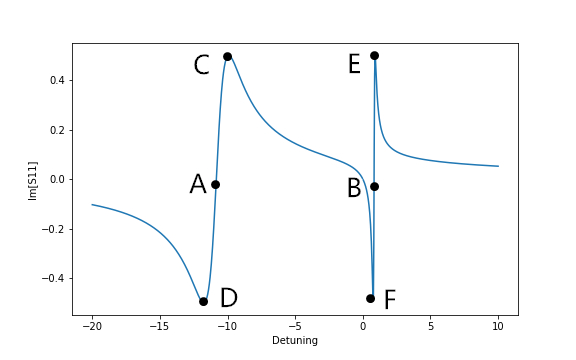
\includegraphics[width=11cm]{pic/3D_cavity/3D_twoCavityResonance.jpg}
     \caption{Dependence of inaginary part of $S_{11}$ on the detuning $\Delta$}
     \label{fig:ImS11}
\end{figure}

Fig\ref{fig:ImS11} is plotted under the condition above. Point A,B in the figure corresponds to two roots for the zero point of $S_{11}$, i.e. $\Delta_2, \Delta_1$ in the text above. Point C, D corresponds to the two peaks sitting around $\Delta_2$, which is the $\Delta_2^1, \Delta_2^2$ in the previous text. The same interpretation also applies to point E, F. From this correspondency we can tell that it is fair to say differnce $|\Delta_1^1 - \Delta_1^2|$ and $|\Delta_2^1 - \Delta_2^2|$ can be interpreted as linewidth of the cavity.

By applying large detuning condition, we can obtain approximation
\\
\begin{equation} \begin{split}
	& \sqrt{\left( \Delta_{fr} \pm \frac{\kappa}{2}\right)^2 + 4 |G| ^ 2} \\
	= & \sqrt{ \Delta_{fr}^2 + \left(\frac{\kappa}{2}\right)^2 \pm 2 \Delta_{fr} \frac{\kappa}{2} + 4 |G| ^ 2} \\
	\approx & \sqrt{ \Delta_{fr}^2 \pm 2 \Delta_{fr} \frac{\kappa}{2} + 4 |G| ^ 2} \\
	\approx & \sqrt{ \Delta_{fr}^2 + 4 |G| ^ 2} \pm \frac{\Delta_{fr}}{\sqrt{ \Delta_{fr}^2 + 4 |G| ^ 2}} \frac{\kappa}{2}
\end{split} \end{equation}
\\
This leads to approximate value of extremum points
\begin{equation} \begin{split}
	\Delta_1^1 = -\frac{1}{2} \Delta_{fr} + \frac{1}{2}\sqrt{\Delta_{fr}^2 + 4|G|^2}  + \frac{\kappa}{4} - \frac{\Delta_{fr}}{\sqrt{ \Delta_{fr}^2 + 4 |G| ^ 2}} \frac{\kappa}{4} \\
	\Delta_1^2 = -\frac{1}{2} \Delta_{fr} + \frac{1}{2}\sqrt{\Delta_{fr}^2 + 4|G|^2}  - \frac{\kappa}{4} + \frac{\Delta_{fr}}{\sqrt{ \Delta_{fr}^2 + 4 |G| ^ 2}} \frac{\kappa}{4} \\
	\Delta_2^1 = -\frac{1}{2} \Delta_{fr} - \frac{1}{2}\sqrt{\Delta_{fr}^2 + 4|G|^2}  + \frac{\kappa}{4} + \frac{\Delta_{fr}}{\sqrt{ \Delta_{fr}^2 + 4 |G| ^ 2}} \frac{\kappa}{4} \\
	\Delta_2^2 = -\frac{1}{2} \Delta_{fr} - \frac{1}{2}\sqrt{\Delta_{fr}^2 + 4|G|^2}  - \frac{\kappa}{4} - \frac{\Delta_{fr}}{\sqrt{ \Delta_{fr}^2 + 4 |G| ^ 2}} \frac{\kappa}{4}
\end{split} \end{equation}
\\
Under the condition where detuning is significantly larger than coupling strength, $\Delta_1$ represents the solution where $\Delta_{rd}$ is small. Thus, we can see it as shifted readout cavity mode. The mode lindewidth
\\
\begin{equation}
	\frac{\delta \omega_1}{2} = |\Delta_1^1 - \Delta_1^2| = \left (1 - \frac{\Delta_{fr}}{\sqrt{ \Delta_{fr}^2 + 4 |G| ^ 2}} \right) \frac{\kappa}{2}
\end{equation}
\\
We can see that the shifted mode gained a finite linewidth due to its hyberdization with leaky Purcell filter mode. Nevertheless, the linewidth is suppressed by the large drtuning. The same interpretation also works for shifted Purcell filter mode
\\
\begin{equation}
	\frac{\delta \omega_2}{2} = |\Delta_2^1 - \Delta_2^2| = \left (1 + \frac{\Delta_{fr}}{\sqrt{ \Delta_{fr}^2 + 4 |G| ^ 2}} \right) \frac{\kappa}{2}
\end{equation}
\\
Which means that shifted Purcell filter mode endures a reduction in the linewidth. If the ratio $\Delta_{fr}/|G|$ goes to infinitely large, two cavity will become completely independent, $\delta \omega_1 \approx 0, \delta \omega_2 \approx \kappa$. This result coincide with our intuition.

It is worthwhile to note that we also obtained relationship
\begin{equation}
	\Delta_1 + \Delta_2 = - \Delta_{fr}
	\label{eq:centerConserved}
\end{equation}
and
\begin{equation}
	\delta \omega_1 + \delta \omega_2 = \kappa
	\label{eq:linewidthConserved}
\end{equation}
Eq\ref{eq:centerConserved} means that the numerical average of two mode frequency is conserved, Eq\ref{eq:linewidthConserved} means that the total linewidth is conserved.

\subsection{Purcell decay rate and readout cavity response}